\chapter{Abbreviations}
\begin{multicols}{2}

\begin{itemize}
    \item API (Application Programming Interface)
    \item ARM (Advanced RISC Machine)
    \item CMOS (Complementary Metal-Oxide-Semiconductor)
    \item FMC (FPGA Mezzanine Card)
    \item FPGA (Field Programmable Gate Array)
    \item GMSL (Gigabit Multimedia Serial Link)
    \item GPU (Graphical Processing Unit)
    \item HD (High Definition)
    \item HDMI (High-Definition Multimedia Interface)
    \item HDR (High Dynamic Range)
    \item $I^2C$ or IIC (Inter-Integrated Circuit)
    \item I/O (Input/Output)
    \item IP (Intellectual Property)
    \item IPv4 (Internet Protokol version 4)
    \item MIPI (Mobile Industry Processor Interface)
    \item MUX (multiplexer)
    \item OpenCV (Open source computer vision)
    \item PC (Personal Computer)
    \item PL (Programmable Logic)
    \item RISC (Reduced Instruction Set Computing)
    \item SZTAKI (Számítástechnikai és Automatizálási Kutatóintézet)
    \item SoC (System-on-Chip)
    \item UAV (Unmanned Aerial Vehicle)
    \item VLSI (Very-Large-Scale Integration)
    \item WXGA (Wide Extended Graphics Array)
    \item RTOS (Real-Time Operating System)
    \item MIT (Massachusetts Institute of Technology)
    \item IoT (Internet of Things)
    \item ROS (Robot Operating System)
    \item MPSoC (MultiProcessor System-on-Chip)
    \item BSP (Board Support Package)
    \item AMP (Asymmetric Multi Processing)
    \item VHDL (VHSIC-HDL) (Very High Speed Integrated Circuit Hardware Description Language)
    \item SDK (Software Development Kit)
    \item HLS (High-level synthesis)
    \item RTL (Register-Transfer Level)
    \item SDSoC (Software Defined System-on-Chip)
    \item CNN (Convolutional Neural Network)
    \item SD (Secure Digital)
    \item VDMA (Video Direct Memory Access)
    \item AXI (Advanced eXtensible Interface)
    \item EAV (End Active Video)
    \item SAV (Strat Active Video)
    \item UDP/IP (User Datagram Protocol / Internet Protocol)
    \item VM (Virtual Machine)
    \item BSP (Board Support Packages)
    \item FPS (frames per seconds)
    \item HWH (HardWare Handout)
    \item XML (eXtensible Markup Language)
    \item LUTs (Look Up Tables)
    \item SI (Single Instruction)
    \item SISD (single instruction stream, single data stream)
    \item RGB (Red Green Blue)
    \item HSV (Hue Saturation Value)
    \item LSI (Linear Space Invariant)
    \item ASIC (Application-Specific Integrated Circuit)
    \item ISA (Instruction Set Architecture)
    \item DSP (Digital Signal Processor)
    \item HBM (High Bandwidth Memory)
    \item ACAP (Adaptive Compute Acceleration Platform)
    \item ReLU (Rectified Linear Unit)
    \item CLB (Configurable Logic Block)
    \item UHD (Ultra-High-Definition)
    \item USB (Universal Serial Bus)
    \item Airsim (Aerial Informatics and Robotics Platform)
\end{itemize}

\end{multicols}


\chapter{Codes related}
\lstset{
    language=Python,
    caption={Error report on the logibrick IP implementation},
    keywordstyle=\color{red},
    stringstyle=\color{blue},
    commentstyle=\color{green},
    morecomment=[l][\color{magenta}]{\#},
    columns=fullflexible,
    breaklines=true,
    postbreak=\mbox{\textcolor{red}{$\hookrightarrow$}\space},
}
\lstinputlisting{assets/xilon_blackbox_error.txt}

\lstset{
    language=Python,
    caption={The Python algorithm main function},
    label={code:original},
    keywordstyle=\color{red},
    stringstyle=\color{blue},
    commentstyle=\color{green},
    morecomment=[l][\color{magenta}]{\#},
    columns=fullflexible,
    numbers=left,
    breaklines=true,
    postbreak=\mbox{\textcolor{red}{$\hookrightarrow$}\space},
}
\lstinputlisting{assets/python_hiba/Original.py}

\lstset{
    language=Python,
    caption={The airsim client class},
    label={code:client},
    keywordstyle=\color{red},
    stringstyle=\color{blue},
    commentstyle=\color{green},
    morecomment=[l][\color{magenta}]{\#},
    columns=fullflexible,
    breaklines=true,
    postbreak=\mbox{\textcolor{red}{$\hookrightarrow$}\space},
}
\lstinputlisting{assets/python_hiba/client.py}

\lstset{
    language=Python,
    caption={Training data generation of the client code},
    label={code:training_data},
    keywordstyle=\color{red},
    stringstyle=\color{blue},
    commentstyle=\color{green},
    morecomment=[l][\color{magenta}]{\#},
    columns=fullflexible,
    breaklines=true,
    postbreak=\mbox{\textcolor{red}{$\hookrightarrow$}\space},
}
\lstinputlisting{assets/python_hiba/get_training_data.py}

\lstset{
    language=Python,
    caption={The decision maker neural network},
    label={code:net},
    keywordstyle=\color{red},
    stringstyle=\color{blue},
    commentstyle=\color{green},
    morecomment=[l][\color{magenta}]{\#},
    columns=fullflexible,
    breaklines=true,
    postbreak=\mbox{\textcolor{red}{$\hookrightarrow$}\space},
}
\lstinputlisting{assets/python_hiba/net.py.txt}


\lstset{
    language=Python,
    caption={The preprocess algorithm},
    label={code:python_preproc},
    keywordstyle=\color{red},
    stringstyle=\color{blue},
    commentstyle=\color{green},
    morecomment=[l][\color{magenta}]{\#},
    columns=fullflexible,
    breaklines=true,
    postbreak=\mbox{\textcolor{red}{$\hookrightarrow$}\space},
}
\lstinputlisting{assets/python_hiba/preproc.py}

\lstset{
    language=C,
    caption={The HLS implementation of the preprocess algorithm},
    label={code:hls_preproc},
    keywordstyle=\color{red},
    stringstyle=\color{blue},
    commentstyle=\color{green},
    morecomment=[l][\color{magenta}]{\#},
    columns=fullflexible,
    breaklines=true,
    postbreak=\mbox{\textcolor{red}{$\hookrightarrow$}\space},
}
\lstinputlisting{assets/preproc_hls/preproc.cpp.txt}

\lstset{
    language=C,
    caption={Test bench source for testing the preprocess HLS block},
    label={code:test_bench},
    keywordstyle=\color{red},
    stringstyle=\color{blue},
    commentstyle=\color{green},
    morecomment=[l][\color{magenta}]{\#},
    columns=fullflexible,
    breaklines=true,
    postbreak=\mbox{\textcolor{red}{$\hookrightarrow$}\space},
}
\lstinputlisting{assets/preproc_hls/preproc_tb.cpp.txt}

\lstset{
    language=C,
    caption={The HLS implementation of the adaptive threshold},
    label={code:adaptive_thrash},
    keywordstyle=\color{red},
    stringstyle=\color{blue},
    commentstyle=\color{green},
    morecomment=[l][\color{magenta}]{\#},
    columns=fullflexible,
    breaklines=true,
    postbreak=\mbox{\textcolor{red}{$\hookrightarrow$}\space},
}
\lstinputlisting{assets/adaptive_thresh/more_adaptive_thrash.cpp.txt}

\lstset{
    language=python,
    caption={Configuration of the Preprocess IP block, and the VDMA},
    label={code:preproc_start},
    keywordstyle=\color{red},
    stringstyle=\color{blue},
    commentstyle=\color{green},
    morecomment=[l][\color{magenta}]{\#},
    columns=fullflexible,
    breaklines=true,
    postbreak=\mbox{\textcolor{red}{$\hookrightarrow$}\space},
}
\lstinputlisting{assets/load_ip.py.txt}

\lstset{
    language=vhdl,
    caption={Conversion from blanking video to BT656},
    label={code:bl2BT},
    keywordstyle=\color{red},
    stringstyle=\color{blue},
    commentstyle=\color{green},
    morecomment=[l][\color{magenta}]{\#},
    columns=fullflexible,
    breaklines=true,
    postbreak=\mbox{\textcolor{red}{$\hookrightarrow$}\space},
}
\lstinputlisting{assets/bl2BT.vhd.txt}

\lstset{
    language=vhdl,
    caption={Conversion from BT656 to blanking video signal},
    label={code:BT2bl},
    keywordstyle=\color{red},
    stringstyle=\color{blue},
    commentstyle=\color{green},
    morecomment=[l][\color{magenta}]{\#},
    columns=fullflexible,
    breaklines=true,
    postbreak=\mbox{\textcolor{red}{$\hookrightarrow$}\space},
}
\lstinputlisting{assets/BT2bl.vhd.txt}

\chapter{Block diagrams}
\begin{figure}
    \centering
    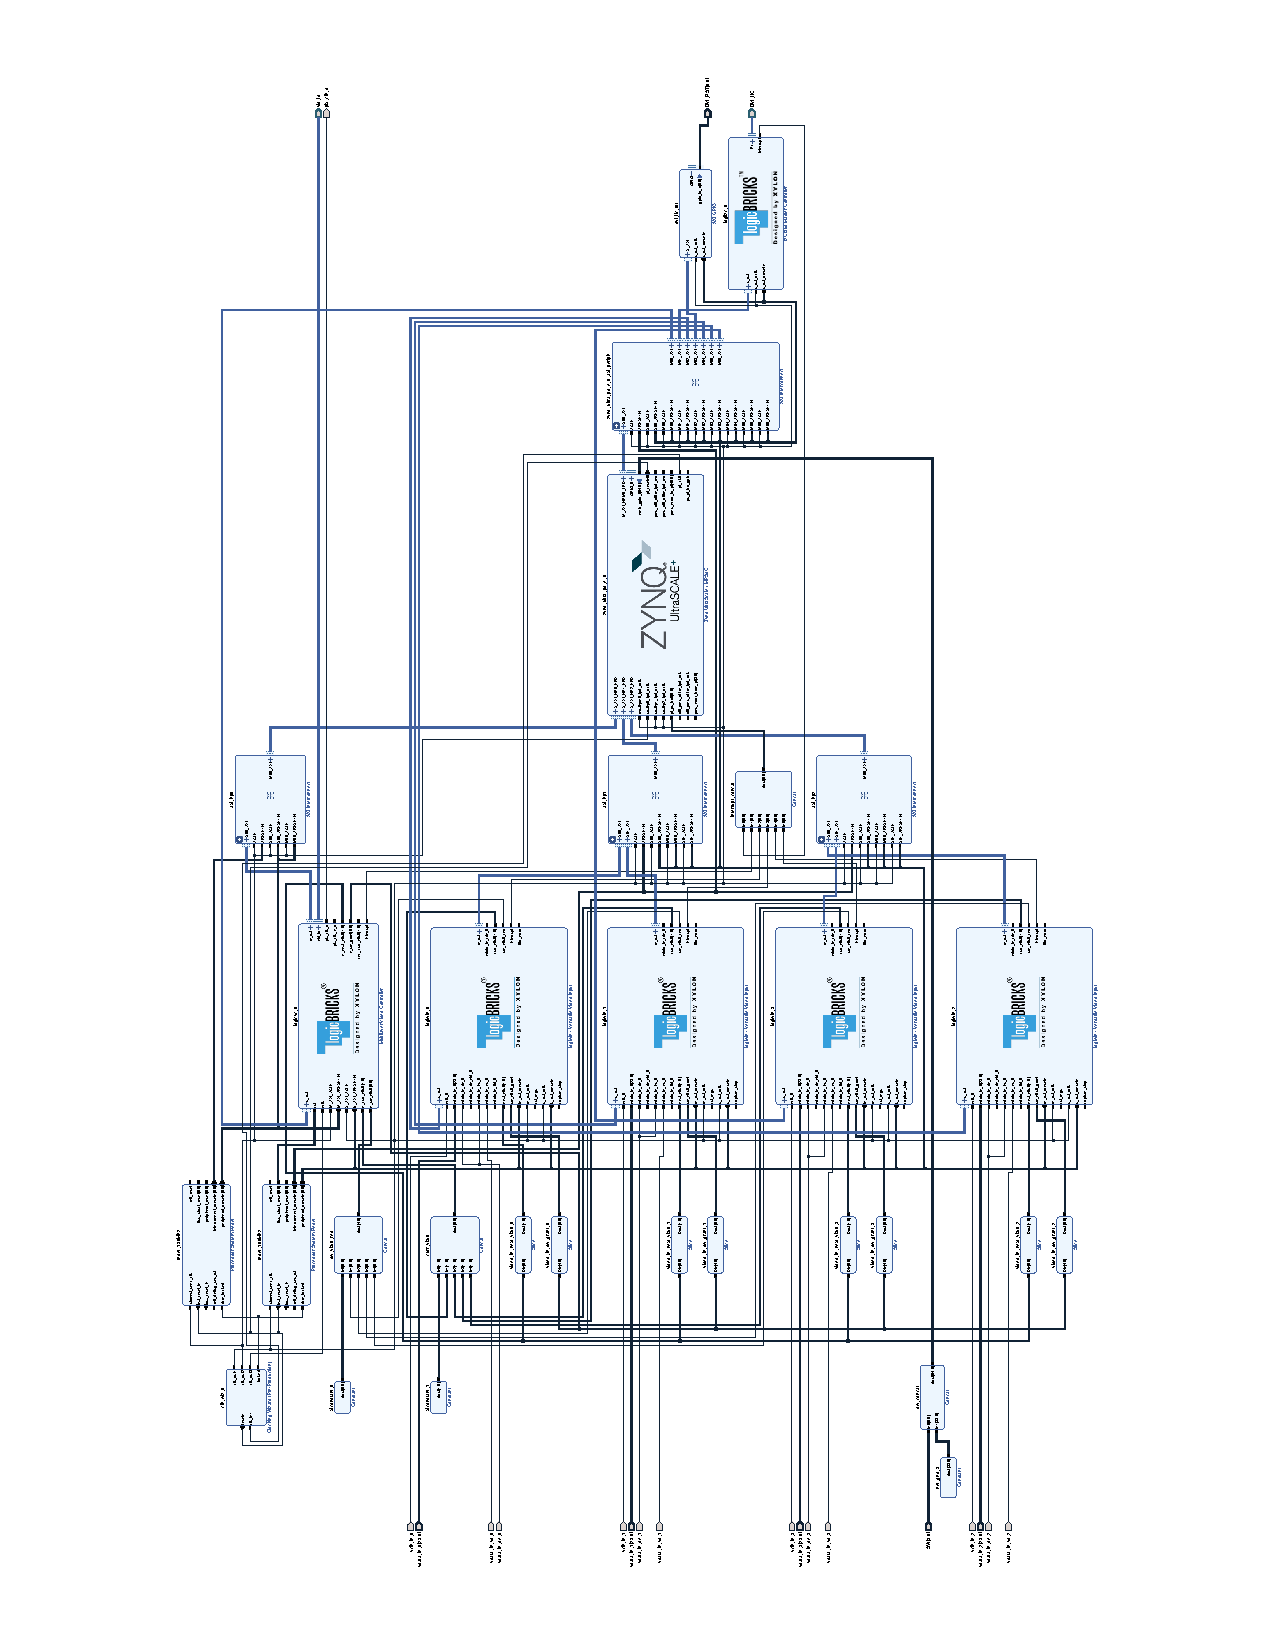
\includegraphics[width=\linewidth]{assets/hp130ac.pdf}
    \caption{Logibricks 4-cam system}
    \label{fig:4_cam_logic}
\end{figure}

\begin{figure}
    \centering
    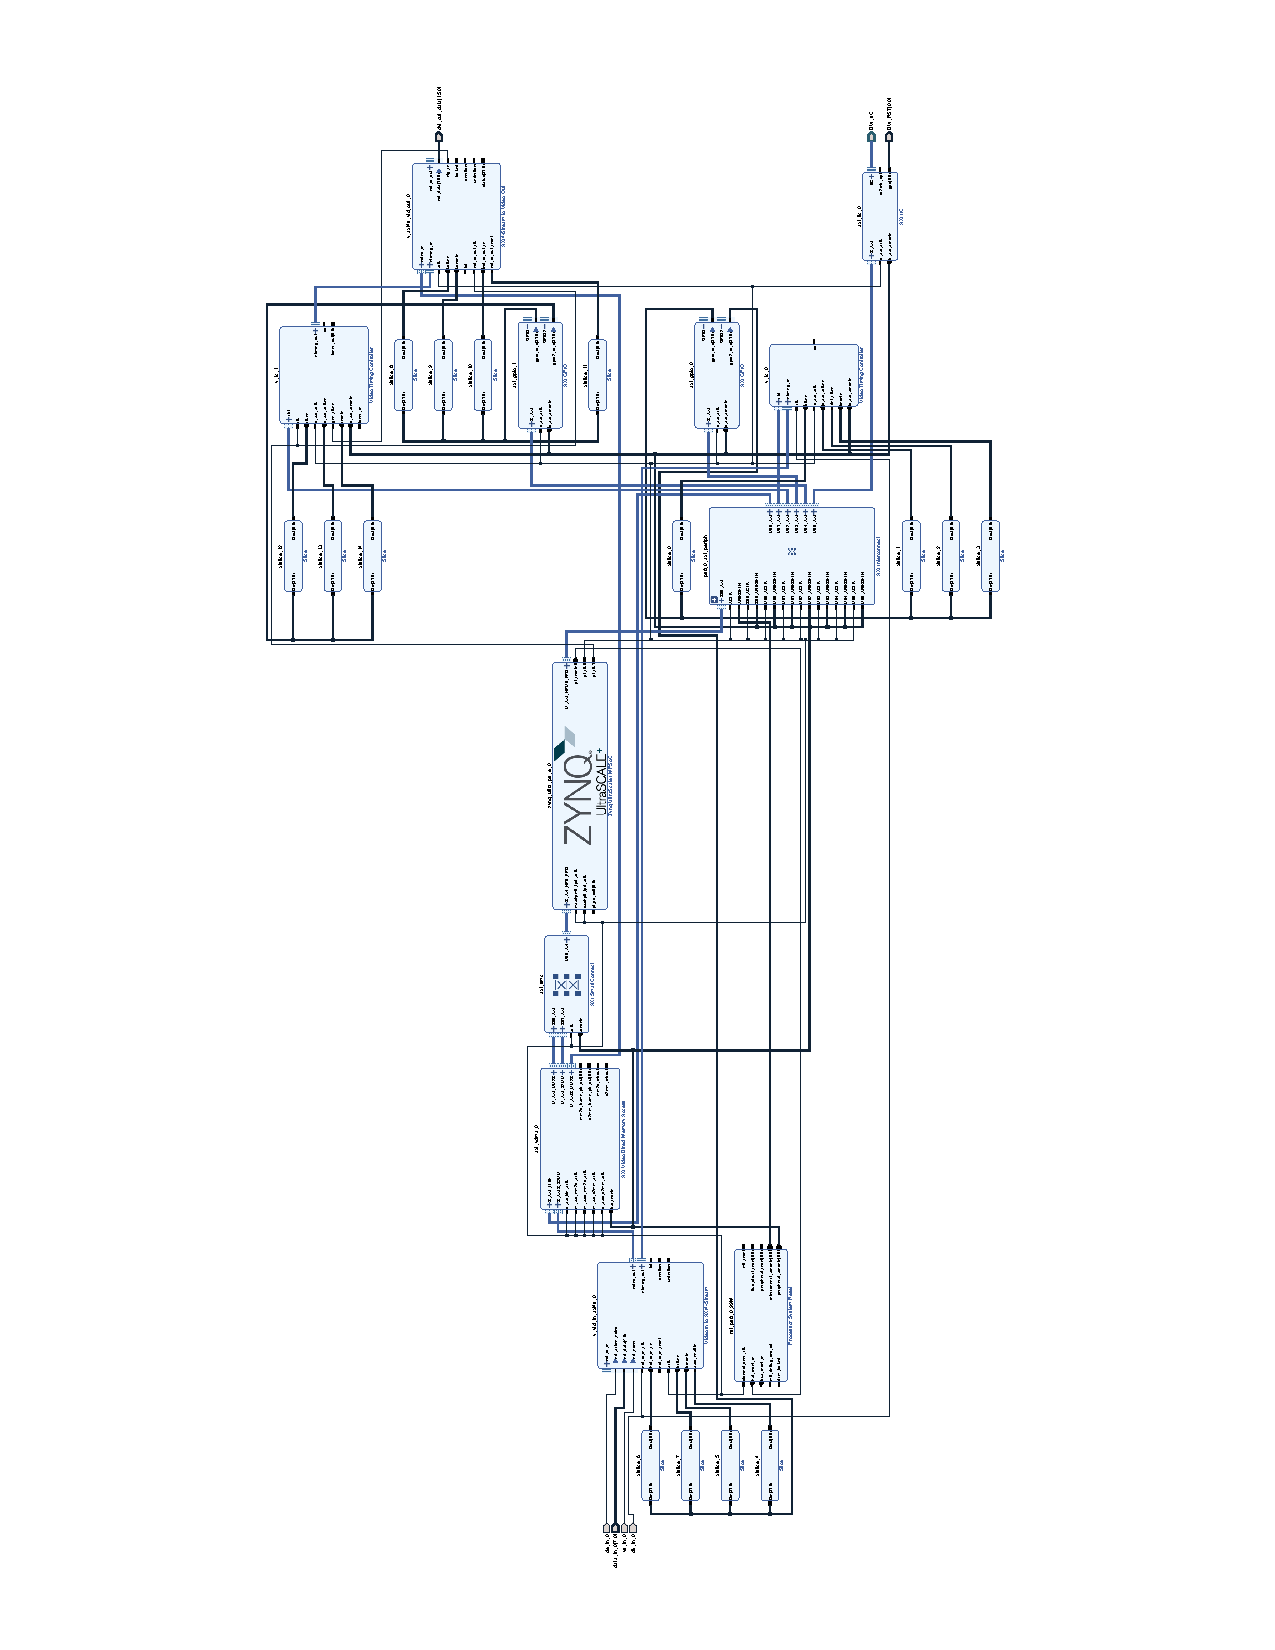
\includegraphics[width=\linewidth]{assets/handmade_1.pdf}
    \caption{Handmade replication of the original}
    \label{fig:4_cam_handmade}
\end{figure}

\begin{figure}
    \centering
    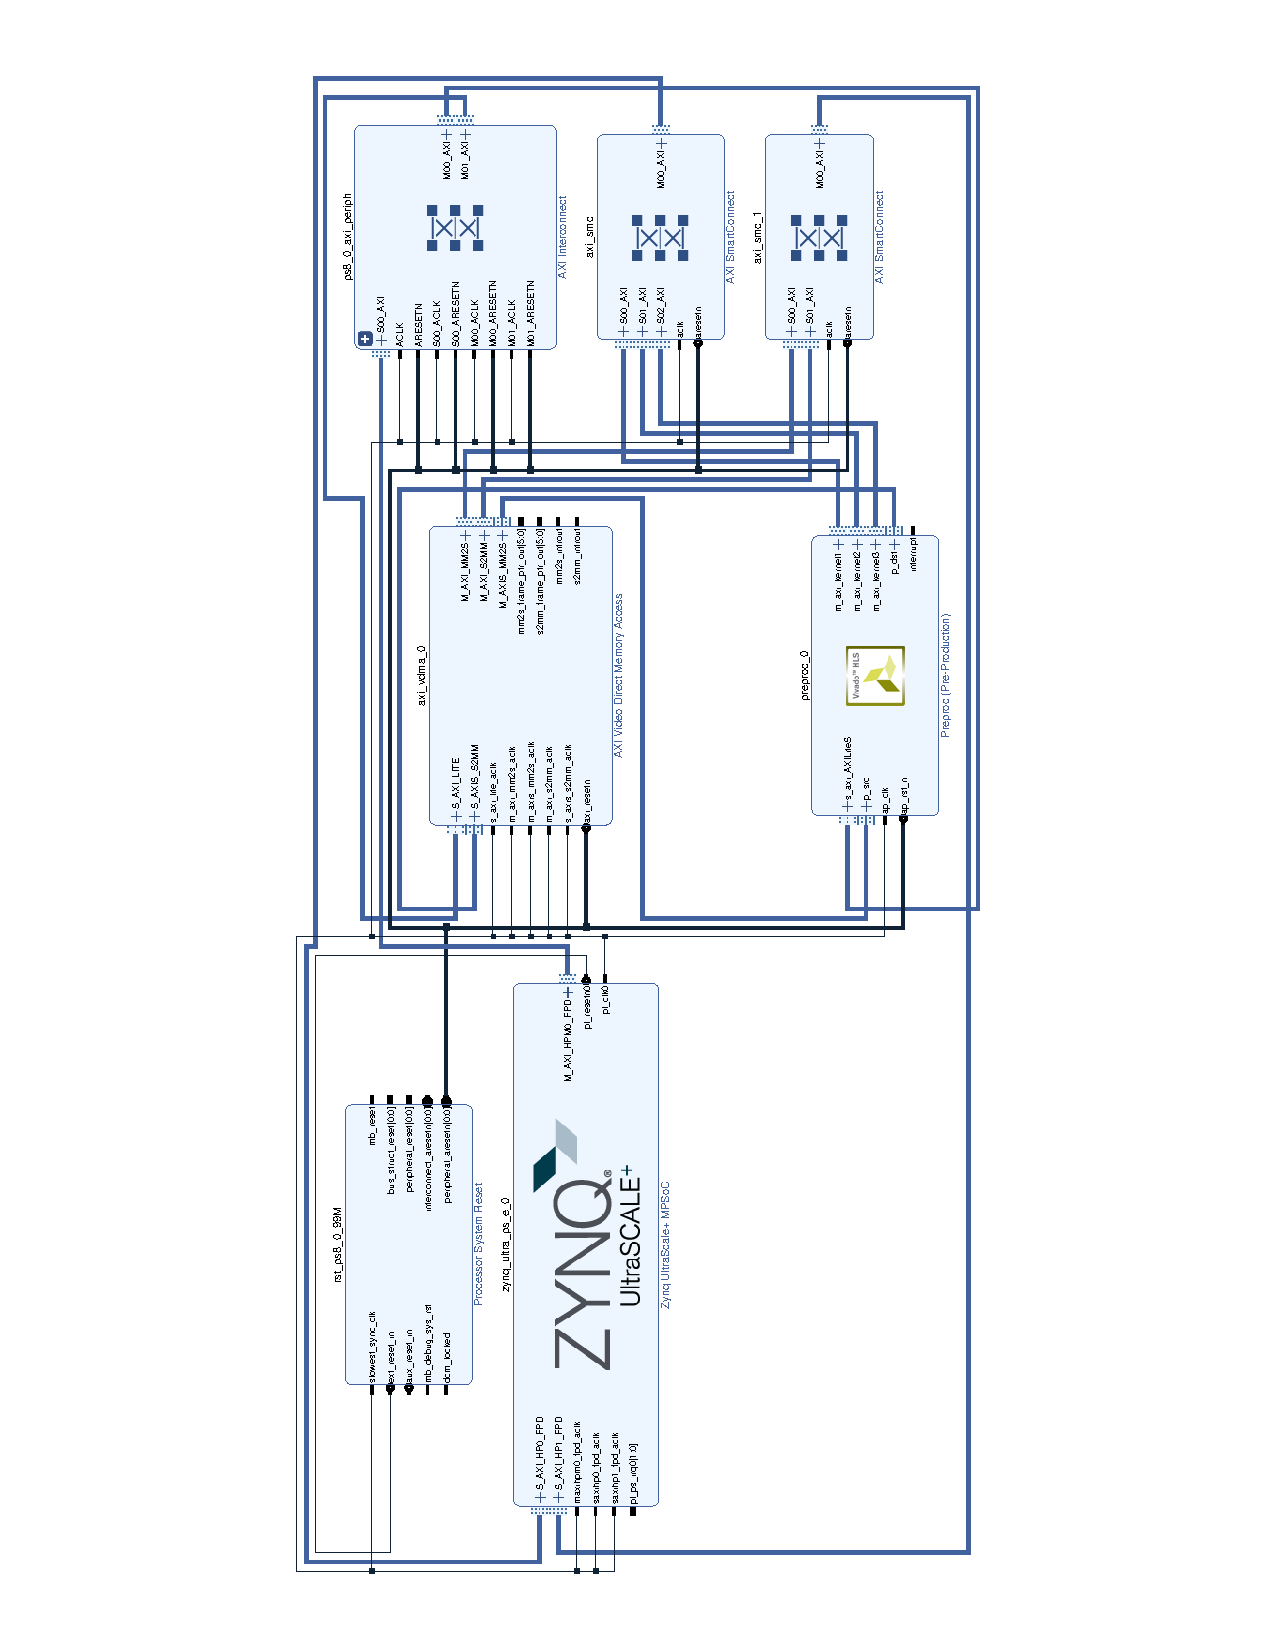
\includegraphics[width=\linewidth]{assets/PreProcess_design.pdf}
    \caption{Block design of the preprocess IP containing the ZYNQ processor sytem, the VDMA and th interconnects}
    \label{fig:block_preproc}
\end{figure}

\begin{figure}
    \centering
    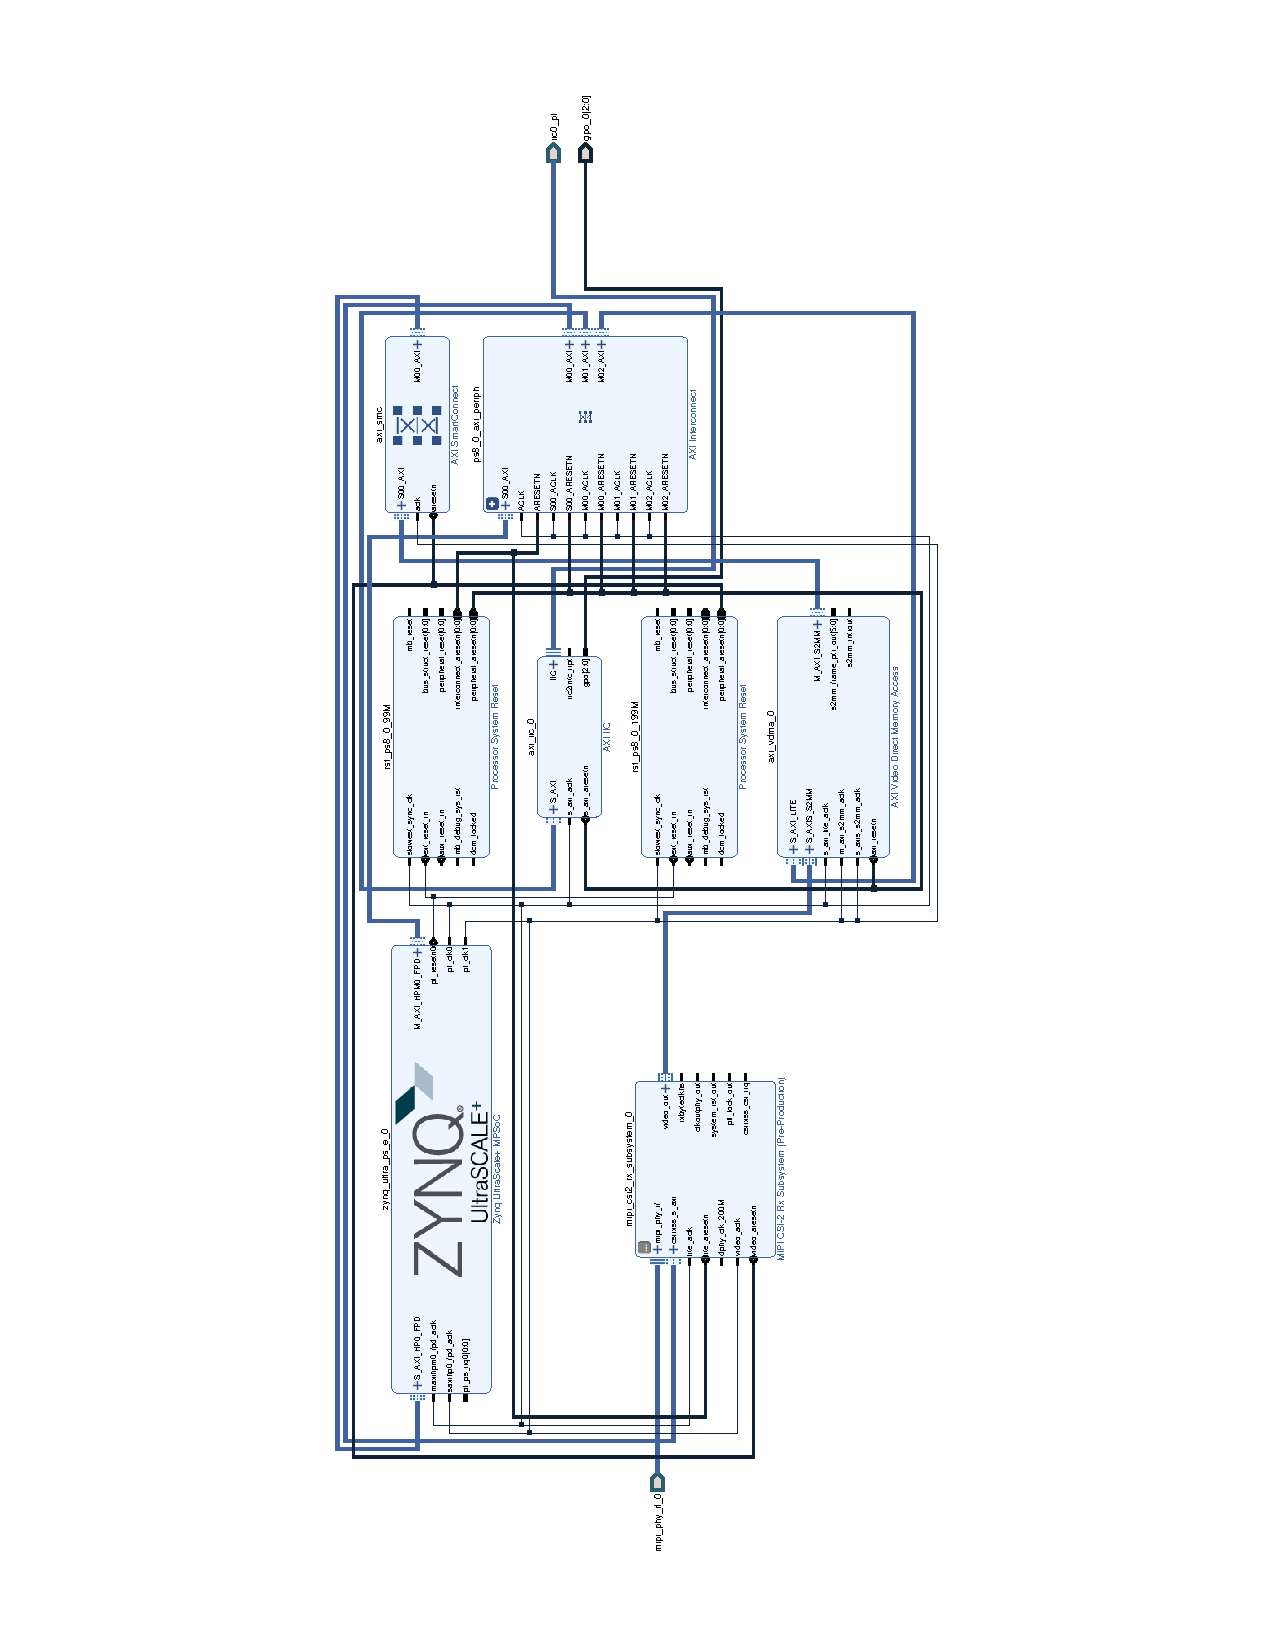
\includegraphics[width=\linewidth]{assets/MIPI_1.pdf}
    \caption{MIPI Rx subsystem with the correspondong blocks}
    \label{fig:block_mipi}
\end{figure}

\chapter{Links}